% ======================================================================
\section{Short horizons and frictions}\label{sec:finite}
% ======================================================================

The results of \cref{sec:lower,sec:exact,sec:cone,sec:fair} describe a regime that \cref{sec:numerics} shows is reached only after about $10^6$ rounds in our own example. A government may get tens of rounds in a policy area. This section says what carries over to short horizons, why the frictions that governments and firms face do not show up in the asymptotic theory, and what a rational planner does in the simplest finite problem.

\paragraph{What carries over.} The identity \eqref{eq:linear}, $\E[R(T)]=D\,\E[n(T)]$, holds for every planner and every $T$. At any horizon, who pays is fixed by which policies are tried and for how long, and a person's cost is their loss under each tried policy times the time it is in force. What does not carry over is the allocation. The asymptotic weights $\cmin_a\propto\Delta_a^{-2}$ come from the requirement of consistency, which says nothing at small $T$. There the natural benchmark is a planner that maximises expected welfare under a prior.

\paragraph{Frictions vanish asymptotically.} A government cannot change policy every round. Changing has a cost, and a policy once adopted stays for a term. In the stochastic bandit neither matters in the limit: with a cost per switch, allocation in growing blocks attains the Lai--Robbins constant with a switching cost of smaller order than $\log T$ \citep{agrawal1988}, and with decisions confined to a small number of batches, of order $\log\log T$, the minimax rate is unchanged \citep{perchet2016,gao2019}. The frictions bite only when the horizon is short, which is one more reason to look there.

\subsection{One status quo, one reform}

The simplest finite problem has a known status quo and a single untried reform. Normalise the status quo's welfare to $0$ per round. The reform's welfare per round is $\theta$, unknown, with prior $\theta\sim\mathcal N(m,1)$, so that welfare is measured in prior standard deviations. While the reform is in force the planner observes $\theta$ plus Gaussian noise of standard deviation $\varsigma$ each round. Policies are held in blocks of $\ell$ rounds (a term), and each change of policy costs $c$. The planner maximises expected total welfare over $T$ rounds, starting from the status quo. We solve the problem numerically by backward induction over the number of rounds the reform has been in force, the posterior mean, and the policy currently in force. We take $\varsigma=3$, so that a single round is weak evidence.

\begin{figure}[t]\centering
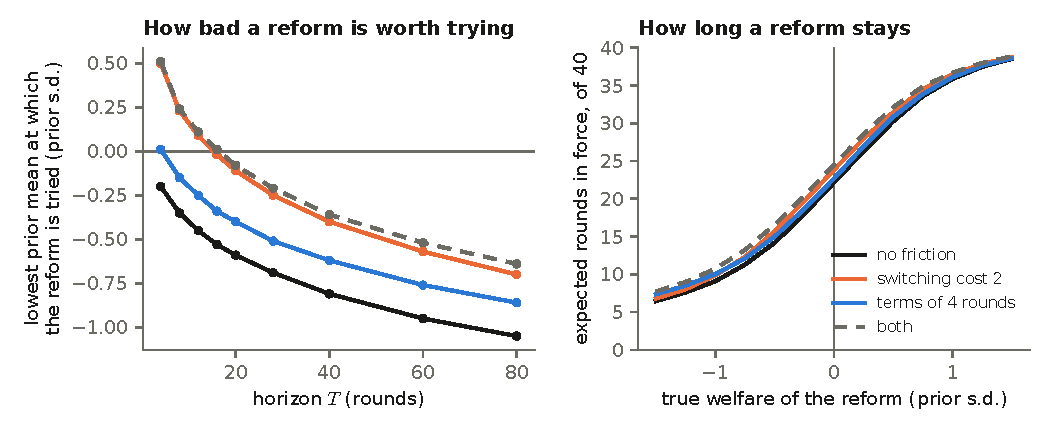
\includegraphics[width=\linewidth]{figures/fig_reform.pdf}
\caption{The one-reform problem with noise $\varsigma=3$. Left: the lowest prior mean $m$ at which the welfare-maximising planner tries the reform. Below zero, the reform is expected to be worse than the status quo. Right: with $T=40$ and $m=0$, the expected number of rounds the reform is in force, as a function of its true welfare (4{,}000 simulated paths per point).}
\label{fig:reform}
\end{figure}

\paragraph{A rational planner tries reforms it expects to be worse.} With no frictions and $T=40$, the planner tries any reform whose prior mean is above $-0.81$ (\cref{fig:reform}, left). It expects such a reform to lose, and tries it because the loss is bounded by the option to stop while the gain, if the reform turns out well, lasts for the rest of the horizon. The threshold falls with the horizon: $-0.20$ at $T=4$, $-0.59$ at $T=20$, $-1.05$ at $T=80$. A planner that tries only reforms it expects to be better than the status quo is leaving welfare unclaimed, and more of it the longer its horizon.

\paragraph{Frictions raise the bar.} A switching cost of $c=2$ moves the threshold at $T=40$ from $-0.81$ to $-0.40$; terms of four rounds move it to $-0.62$. At $T=4$ a term of four rounds removes the option to stop altogether, and the planner tries the reform only if it expects it to be better. With a switching cost the reform must also repay the cost, so the threshold at $T=4$ is $+0.5$. Frictions also keep reforms in force longer once tried, though the effect is small here (\cref{fig:reform}, right): the main effect of commitment and inertia is on which reforms are tried at all.

\paragraph{Bad reforms are tried, and somebody pays.} With $m=0$ and $T=40$, a reform whose true welfare is $-0.5$ stays in force for $14$ rounds on average, and one at $-1$ for $9$. This is the planner working as intended, and the people who lose under that reform bear the cost for those rounds. With a single reform the regret vector lies along one direction: person $i$ loses $\mu_{i,a_0}-\mu_{i,\text{reform}}$ per round for as long as the trial lasts. The per-person question at a short horizon is therefore less about how to split exploration between arms and more about three things the planner controls: which reforms are put on the agenda, how quickly a failing one is stopped, and whether its losers are compensated for the rounds it ran.

With several untried reforms the order in which they are tried decides who pays first, and under a short horizon some will never be tried. We leave that problem open.
